In this section the basic concepts of process mining, long short-term memory networks, text mining as well as necessary formal definitions and notations are defined.


\begin{figure}
	\centering
	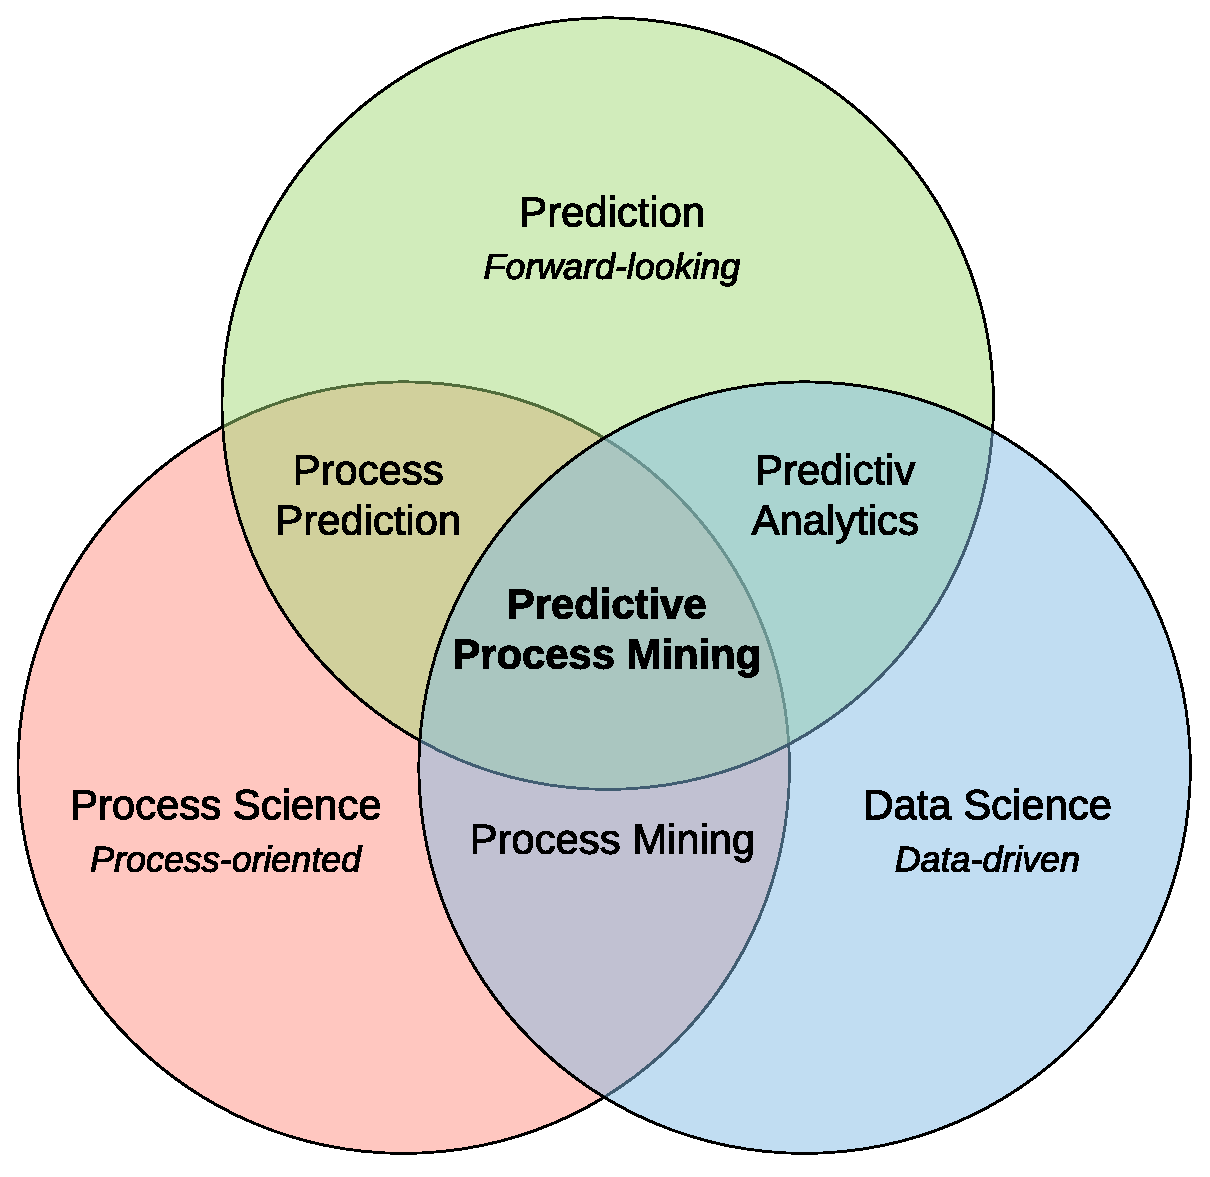
\includegraphics[width=0.5\textwidth]{figures/predictive-process-mining}
	\caption{Predictive Process Mining combines the concepts of process science, data science and prediction}
\end{figure}


\section{Processes, Event Logs, Process Mining, }

A (business-)process is a collection of activities that are performed in a specific order to archive a goal.
Each performed activity belongs to specific case and is completed at a certain time \cite{DBLP:conf/bpm/AalstAM11}.
A case can be e.g. a patient in a hospital, a customer of a company or an order and is usually identified by an ID, while 
the time is specified by a timestamp.
Each execution of a process refers to exactly one case.
The trinity of case, activity and timestamp is called event.
An event can have more attributes depending on the context, like resource, cost or transactional information.

If the execution of a process is logged by an information system, the resulting event data is called event log.
The event log is a set of events, that are usually grouped by their case ID. Depending on the format of the event log, it can also contain additional data on case level.
Most common formats for event logs, which are not part of an database, are comma-separated values (CSV) and eXtensible Event Stream (XES) \cite{DBLP:conf/caise/VerbeekBDA10a}.

Process mining is the discipline that covers all approaches aiming to generate value out of event data.
As an umbrella term, Process Mining comprises or utilizes concepts of Business Process Management (BPM), Data Mining, Business Process Intelligence (BPI), Big Data, Workflow Management (WfM), Business Activity Monitoring (BAM) \cite{DBLP:books/sp/Aalst16} as well as Machine Learning (ML) \cite{DBLP:conf/bpm/VeitGMHT17}.

Process mining can be divided into a set of subdisciplines mainly process discovery, conformance checking, process enhancement and process analytics \cite{DBLP:conf/caise/EckLLA15}.
Process discovery aims to generate process models out of event data in order to understand a process and enable further analysis.
Conformance checking is about comparing the intended and observed behavior of a process. 
On top of these diagnostic approaches, process enhancement deals with the improvement of processes.

Driven by the fast and ongoing development of quantitative prediction methods in data science and machine learning, prediction-based methods have been applied to event data leading to process prediction, a major subject in process analytics.
Forecasting the future of a running process instance is the main goal in process prediction and also the main topic of this thesis.



\section{Basic notations, Sequences, Functions}

The set $\mathbb{N}$ denotes the set of all natural numbers $\{1, 2, 3, \dots\}$ while $\mathbb{N}_0 = \mathbb{N} \cup \{0\}$ denotes the set of natural numbers including 0.
Given a set $A$, $A^n$ describes the set of all sequences $\langle a_1, a_2, \dots, a_n\rangle$ over $A$ of length $n$ with $a_i \in A$, $1 \leq i \leq n$.
The set $A^0$ is defined as $\{\langle \rangle\}$, where $\langle \rangle$ is the empty sequence of length $0$.
The set of all possible sequences over $A$ is given with $A^* = \bigcup\limits_{i\in \mathbb{N}_0} A^i$.



\section{Events and Traces}

\begin{definition}
An  $event$ is defined by tuple $e = (a,c,t,d_1,\dots, d_m) \in \mathcal{C} \times \mathcal{A}  \times \mathcal{T} \times \mathcal{D}_1 \times \dots \times \mathcal{D}_m =  \mathcal{E}$ where  $c \in \mathcal{C} $ is the case id, $a \in \mathcal{A}$ is the executed activity and $t \in \mathcal{T}$ is the timestamp of the event.
Furthermore, each event contains a fixed number $m \in \mathbb{N}_0$ of additional attributes $d_1 \dots d_m$ in their corresponding domains $\mathcal{D}_1, \dots , \mathcal{D}_m$.
In case that no additional attribute data is given ($m = 0$) the event space $\mathcal{E}$ is reduced to $\mathcal{C} \times \mathcal{A}  \times \mathcal{T}$.
\end{definition}

Throughout this thesis,  $\mathcal{C} = \mathbb{N}_0$, $|\mathcal{A}| < \infty$ and $ \mathcal{T} = \mathbb{R}$ is assumed, where $t \in \mathcal{T}$ is given in Unix time, precisely the number of seconds since 00:00:00 UTC on 1 January 1970 minus the applied leap seconds.
Each additional attribute is assumed to be numerical, categorical or textual, i.e. $D_i = \mathbb{R}$, $|D_i| < \infty$ or $D_i = \Sigma^\ast$  for $1 \leq i \leq m$ and some fixed Alphabet $\Sigma$.

\begin{definition}
	A $trace$ is a finite and non-empty sequence of events $\sigma = \langle e_1, e_2, \dots\rangle \in  \mathcal{E}^\ast$ with increasing timestamps, i.e. $\pi_\mathcal{T} (e_i) < \pi_\mathcal{T} (e_j) $ for $1 \leq i < j \leq |\sigma|$.
\end{definition}




\section{Long short-term memory networks}

Long short-term memory (LSMT) is an advanced recurrent neural network architecture originally presented by \citeauthor{DBLP:journals/neco/HochreiterS97} in \citeyear{DBLP:journals/neco/HochreiterS97}  \cite{DBLP:journals/neco/HochreiterS97}.
This approach addresses the well-known vanishing and exploding gradient problem \cite{DBLP:conf/icml/PascanuMB13}  of traditional recurrent neural networks by introducing more complex LSTM cells as hidden units.
The proposed architecture has been significantly improved several times with the introduction of forget gates \cite{DBLP:journals/neco/GersSC00} and the removal of output activation functions \cite {DBLP:journals/tnn/GreffSKSS17}.
Although LSTM networks have been available for a long time, the breakthrough of this technology is dated around 2016 after many success stories of LSTM in combination with large data sets and GPU hardware have been reported for sequence to sequence tasks like text translation \cite{DBLP:journals/corr/WuSCLNMKCGMKSJL16}.


Gated recurrent units (GRU) \cite{DBLP:conf/emnlp/ChoMGBBSB14} are the competing gating mechanism by \citeauthor{DBLP:conf/emnlp/ChoMGBBSB14} that have fewer parameters and perform similar to LSTM.
However, more recent studies show, that LSTM outperforms GRU consistently in neural machine translation tasks \cite{DBLP:journals/corr/BritzGLL17}.

Basic feedforward neural networks comprise an input layer, arbitrarily many hidden layers and an output layer.
Each layer consists of cells that compute and output the weighted sum of the cells of the previous layer that has been passed to an activation function.


Recurrent neural networks extend traditional feed forward networks with backfeeding connections between hidden cells.
This allows the network to keep a state across inputs and makes the neural network ready to process arbitrarily long sequences of input data.

In LTSM networks the hidden cells are replaced with more complex LSTM cells.
These cells uses as input the state $C_{t-1}$ and the output $h_{t-1}$ of the cell in the previous time step and the output of the previous layer.
Each LSTM cell produces an output $h_t$ and state $C_t$.


\begin{equation}\label{key}
	f_t = \sigma(W_f \cdot [h_{t-1}, x_t] + b_f)
\end{equation}

\begin{equation}\label{key}
	i_t = \sigma (W_i \cdot [h_{t-1}, x_t] + b_i)
\end{equation}

\begin{equation}\label{key}
	\bar{C} = \tanh (W_C \cdot [h_{t-1}, x_t] + b_C)
\end{equation}

\begin{equation}\label{key}
	C_t = f_t \times C_{t-1} + i_t \times \bar{C}_t
\end{equation}

\begin{equation}\label{key}
	o_t = \sigma (W_o \cdot [h_{t-1}, x_t] + b_o)
\end{equation}

\begin{equation}\label{key}
	h_t = o_t \times \tanh(C_t )
\end{equation}


\section{Text mining}

Text mining describes all techniques to generate value out of unstructured or semi-structured textual data.


$\diff$